\chapter{Foam Working Training} \label{foam_training}

\section{Introduction}

This training will cover the basics about how to create a project out of foam. Best practices on how to properly use adhesives, cut and shape foam, and coat foam will be covered to ensure an adequate knowledge of foam working.
\section{Hazards}

The following is possible hazards when working with foam and any of the equipment used on the foam.  Please take note of these hazards and make sure you understand the possible dangers and the steps needed to reduce possible harm to yourself.

\begin{framed}
\begin{wrapfigure}{L}{0.15\linewidth}
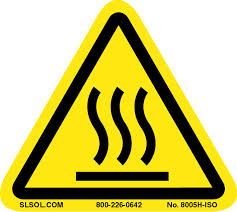
\includegraphics[width=\linewidth]{images/burn_hazard.jpg}
\end{wrapfigure}
\ \\
Several tools used to shape and cut foam use heat to melt the foam. In order to reduce burn risk, keep appendages away from the heat source and handle hot tools and materials with care. Always be familiar with safety and operating procedures of the tool being used in order to minimize burn risks. Always be aware of your surroundings and others while working with hot tools and materials.
\end{framed}
\ \\
\begin{framed}
\begin{wrapfigure}{L}{0.15\linewidth}
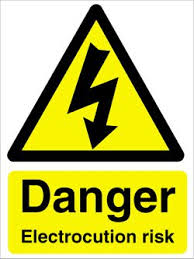
\includegraphics[width=\linewidth]{images/electrocution_hazard.jpg}
\end{wrapfigure}
\ \\
Some of the tools used while shaping foam require power to operate. These tools can result in electrocution if used improperly. Always check cords on plugged in equipment for damage prior to use. Do not use a piece of equipment that has a damaged or frayed cord. Report any damage to a lab monitor immediately. Always ensure that when plugging in equipment, the plug is fully inserted into the outlet and has a snug fit. Cords that are not securely plugged in present a potential electrocution hazard.
\end{framed}

\begin{framed}
\begin{wrapfigure}{L}{0.16\linewidth}
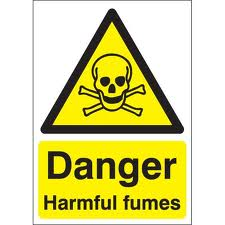
\includegraphics[width=\linewidth]{images/fumes_hazard.jpg}
\end{wrapfigure}
\ \\
Shaping foam can result in fumes. These fumes are not dangerous in the quantities seen while cutting foam correctly. In order to reduce any possible adverse effects, however, use a ventilation system when possible. Avoid excessive heat while cutting foam as the higher the temperature, the higher the quantity of fumes created. If nausea or light-headedness occur as a result of foam fumes, report it to a lab monitor and they will help you get to fresh air.
\end{framed}

\begin{framed}
\begin{wrapfigure}{L}{0.15\linewidth}
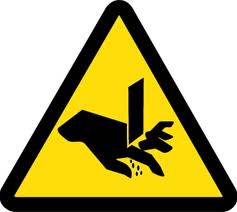
\includegraphics[width=\linewidth]{images/cut_hazard.jpg}
\end{wrapfigure}
\ \\
Hobby knives and other such tools used to shape foam have the potential to cause injury if used carelessly or improperly. Having the appropriate training that each tool requires is the best way to minimize the risk of cuts. Always make sure that your immediate surroundings are cleared of potential hazards and other people before using cutting tools as this helps reduce the risk of injury to both yourself and others. Always cut away from yourself and bystanders. Do not wear loose fitting clothing as this can be caught in the cutting tool and cause injury.  
\end{framed}

\subsection{Chemicals}
Chemicals have the potential to cause injury from mild skin and eye irritation to severe burns and potentially death. In order to minimize this risk, be familiar with the chemical prior to use. Read and follow all safety information listed on the chemical. Always use a proper vent hood when dealing with chemicals that create harmful fumes.

\section{Foam Safe Adhesives}
There are many different adhesives which can be used with foam.  Some work well, others do not. Many types of adhesives can produce toxic fumes and must be handled with care.  Always consult with a lab monitor before using an adhesive that you are not familiar with.
\subsection{Epoxy}
Epoxy is acceptable for almost any foam gluing application.  It is available in fast and slow curing times.  Epoxy is a high strength resin based adhesive, and can act as a structural glue.  Epoxy should be used for most foam constructions.  However, it is not very sandable.
\subsection{Foam Safe CA}
Foam safe CA (cyanoacrylate), as the name implies, is a super glue that is safe for foam.  It comes in several different viscosities, and is sometimes referred to as “odorless” CA.  CA accelerator can be sprayed on the adhesive for instant curing.  Foam safe CA works well for joining foam surfaces, and is not sandable
\subsection{Foam Fusion}
Foam Fusion is a type of adhesive for EPS foam.  It has a long cure time, but is sandable and hotwire safe.  In house tests have shown this adhesive to be stronger than the foam itself.
\subsection{Hot Glue}
Hot glue, which can be used on several types of foam, is not recommended for construction.  It is very low strength, and does not soak into the foam, creating a very weak joint.  Hot glue can also melt into the foam, for some types of foam, if hot glue must be used, a low temp glue should be used with the appropriate gun set to low temperature.  Hot glue is also not sandable, and will cause valleys to be formed around the joint if attempted.  Again, hot glue is not a structural adhesive, and therefore should not be used on high stress joints, such as wing spars, wing saddles, wing butt joints, and empennage attachments on aircraft.  Consult a lab monitor for advice on proper glue joint practices and applications.
\section{Cutting/Shaping Foam}
Cutting and shaping foam can be done in a variety of different ways. The most common are using a hot wire cutter, using a hot knife, or using a hobby knife.  The M:2:I Lab has hot wire and hot knife cutters that can be used for this purpose.  The following goes into instructions on using these tools with foam.

\chapter{Hot wire Cutters}
A hot wire cutter utilizes a heated wire to precisely melt foam. This is accomplished by running electricity through a relatively thin wire. As the current passes through the wire, the wire heats up. Most hot wire cutters have a unit that regulates the current passing through the wire in order to adjust the heat that the wire is producing. There are several types of hot wire cutters that this lab uses.

\section{Vertical Hot Wire Cutting Station}
\begin{framed}
\begin{wrapfigure}{L}{0.15\textwidth}
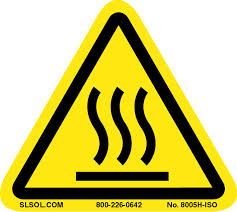
\includegraphics[width=.7in]{images/burn_hazard}
\end{wrapfigure}
\ \\
The wire on the foam cutter can reach high temperatures that can cause severe burns.  Care should be taken at all times when using the vertical cutter to avoid possible burns.
\end{framed}

\begin{framed}
\begin{wrapfigure}{L}{0.15\textwidth}
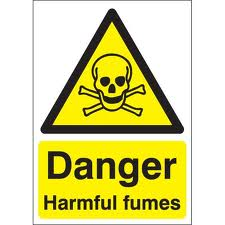
\includegraphics[width=.7in]{images/fumes_hazard}
\end{wrapfigure}
\ \\
Depending on the foam and if any hot wire safe adhesive is used fumes may be generated from using the hot wire cutter.  Make sure any adhesive you use is safe for hot wire cutting and minimize exposure to any fumes generated during cutting.
\end{framed}

The vertical hot wire station shown in Figure \ref{fig:verthotwire} uses a vertical wire that is set perpendicular to the work surface to cut out shapes from foam. This station ensures that the cut has as little taper to the cut as possible. In addition, the table also has slots set up for a mobile fence to ensure that straight cuts can be made from virtually any angle.

\begin{figure}[ht]
\centering
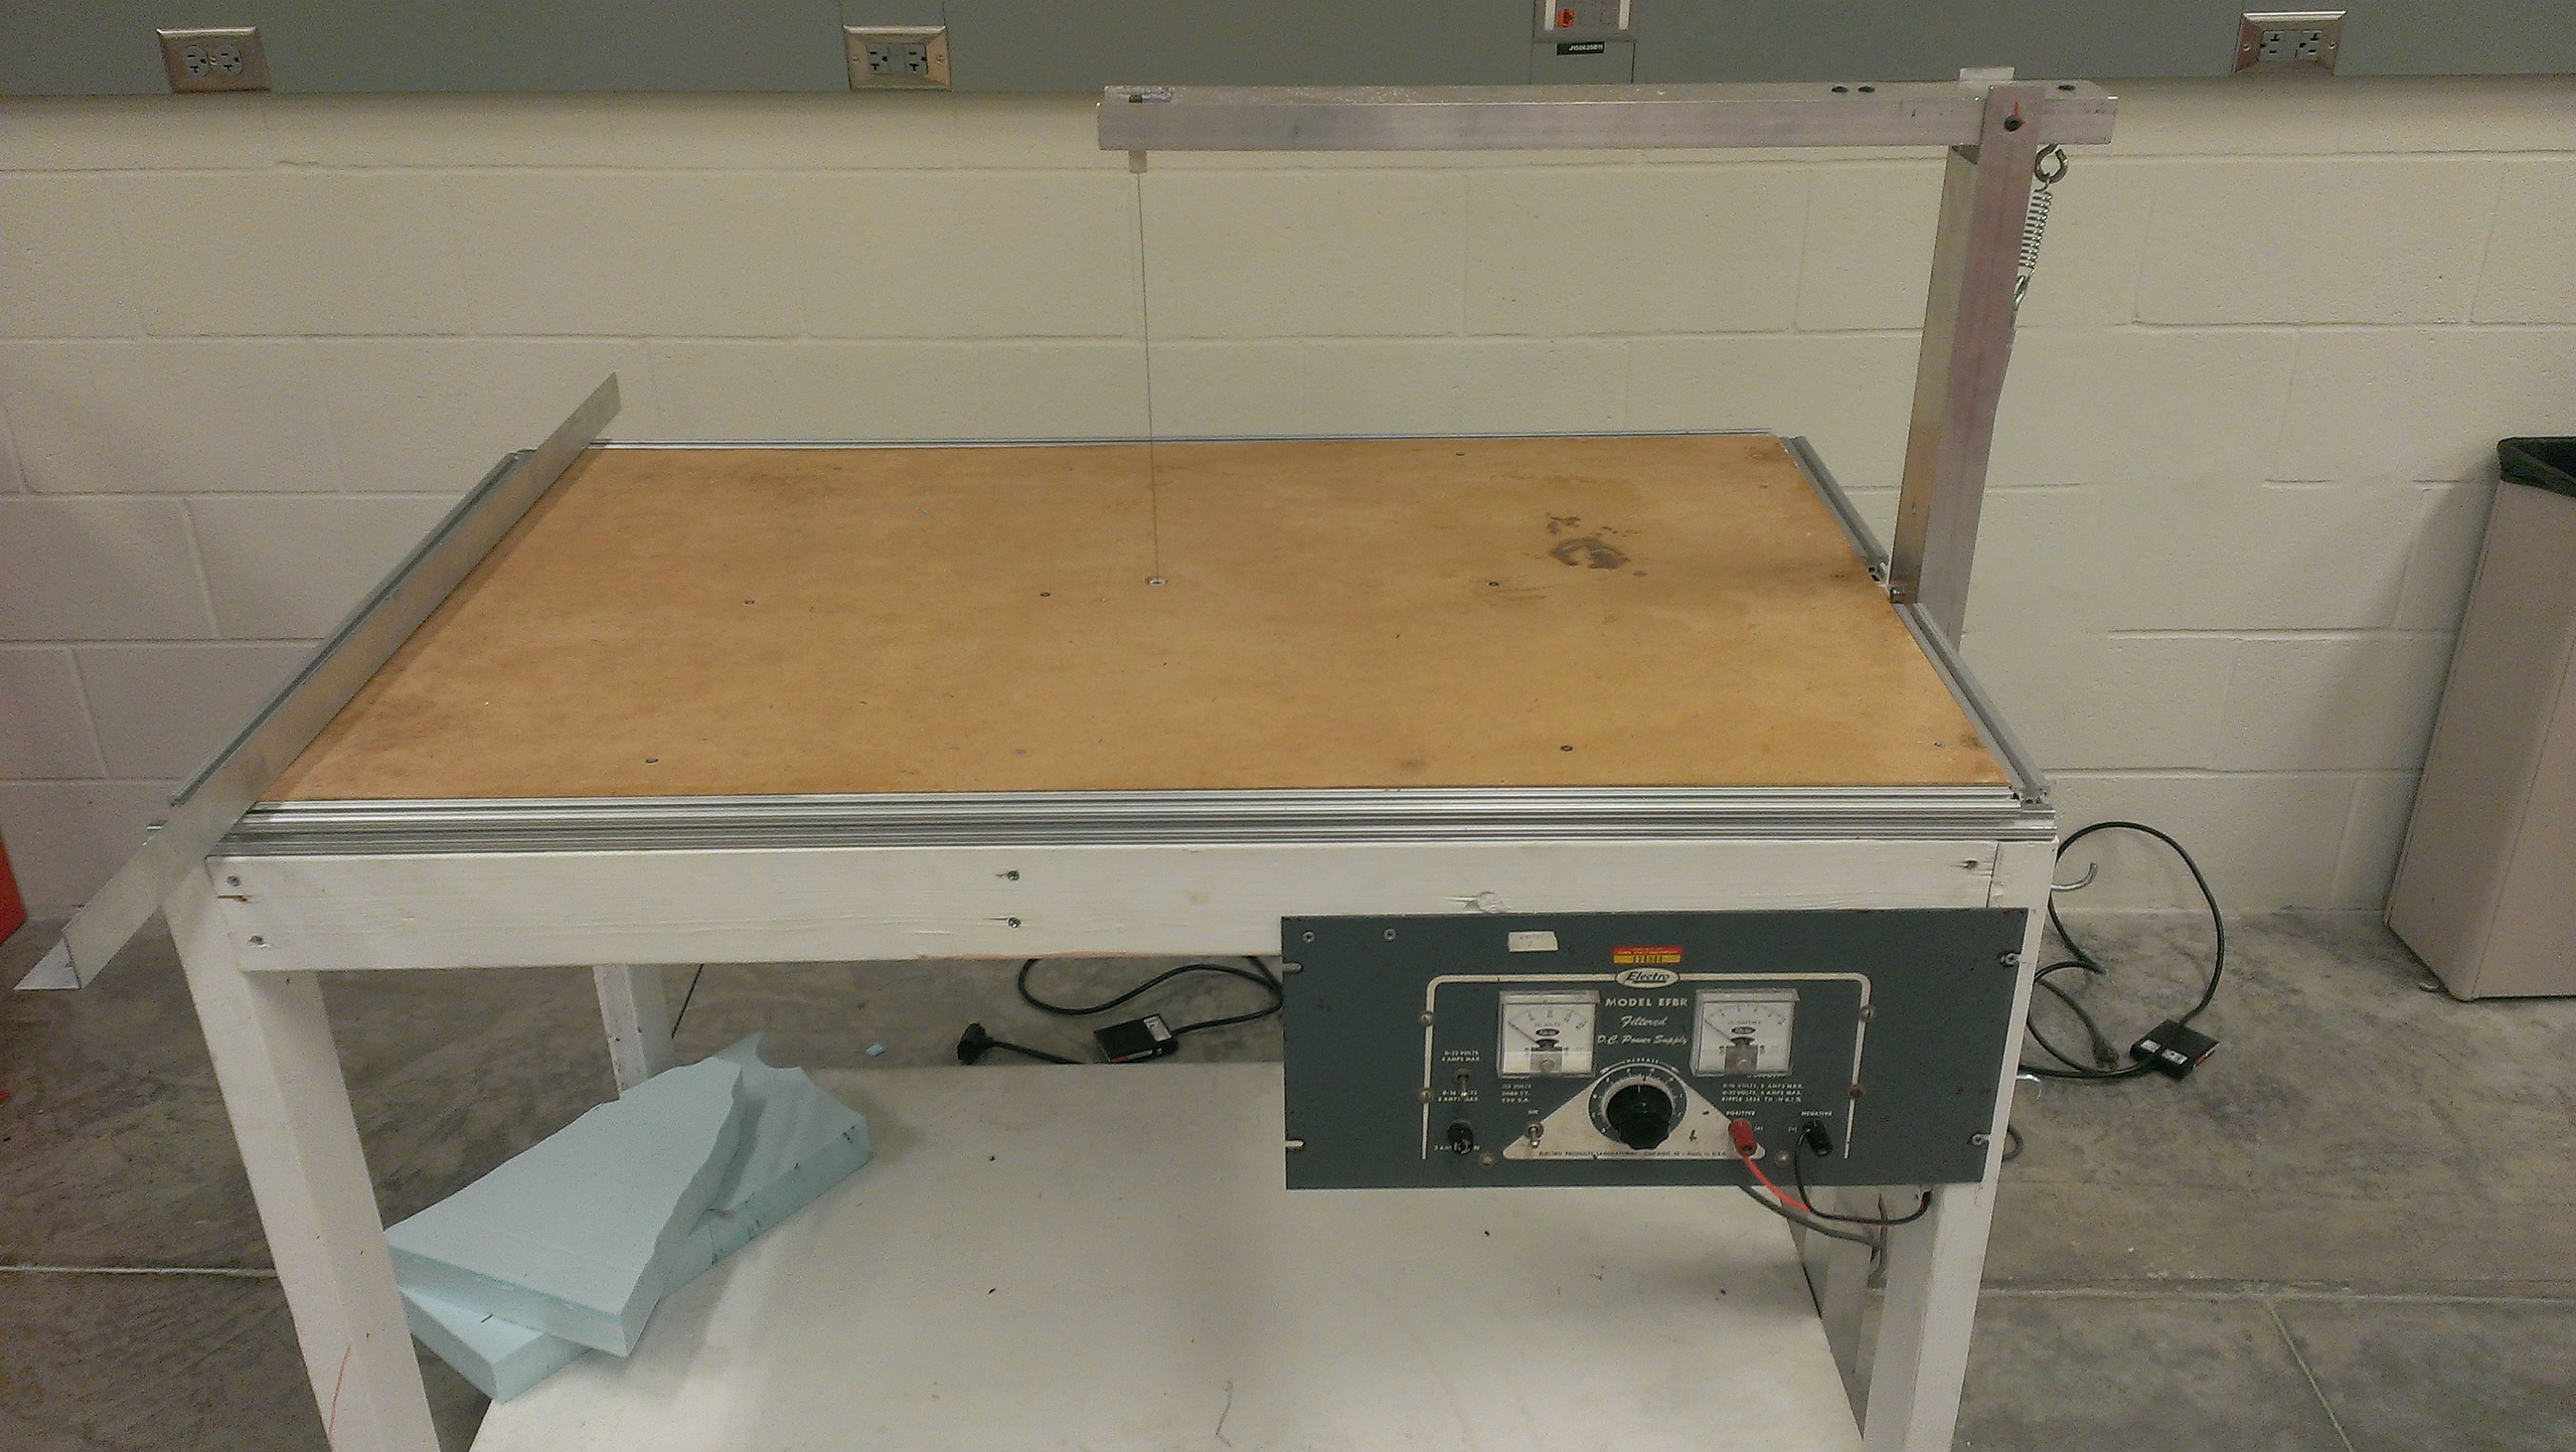
\includegraphics[width=4in]{images/IMAG0198}
\caption{Vertical Hot Wire Cutting Station}
\label{fig:verthotwire}
\end{figure}

\subsection{Operation}
To use the vertical hot wire cutting station, follow these instructions.

%\begin{figure}[h]
%\centering
%\includegraphics[width=2in]{../images/IMAG0222}
%\caption{Power and Heat settings on the power supply}
%\label{fig:hotwirepower}
%\end{figure}
\begin{enumerate}
\item Turn the Power setting to ON
\item Set the Heat Setting to the appropriate level
\begin{enumerate}
\item Turn clockwise to increase the heat output
\item Start on the lowest setting and slowly increase until the wire starts cutting smoothly
\item The correct heat setting will partially depend on travel speed. The higher the travel speed, the higher the heat setting can be set
\item The ideal cutting temperature is one in which the lag seen in the wire and the excess melting is minimized, a bow in the wire is due to the wire being too cold or the travel speed to fast
\end{enumerate}
\item When the wire has heated up, proceed to cut out the desired profile
\begin{enumerate}
\item To cut material, slide the work piece on the tabletop and slide the material into the heated wire at the cut location, use a slower pace in order to prevent the wire from being pulled
\item Vary the rate of travel to minimize wire lag and overheating the material
\end{enumerate}
\item Turn the power off after completing all cuts
\item Unplug cord and wrap up on the cord posts
\item Clean up immediate work area
\begin{enumerate}
\item Small, unusable foam scraps need to be thrown away
\item Excess usable foam scraps can be kept on the bottom shelf of the hot wire table
\item Sweep and vacuum after each use of the hot wire table
\end{enumerate}
\end{enumerate}

Too fast of a travel speed will result in pulling the wire or wire lag. This leads to less precise cuts. Cutting at a slower speed will help to minimize the lag and maximize the accuracy of the cut.

%\begin{figure}[h]
%\centering
%\includegraphics[trim = 0mm 50mm 0mm 750mm,clip,width=2in]{../images/IMAG0223}
%\includegraphics[width=2in]{../images/IMAG0224}
%\caption{The picture on the left shows a nice clean cut with the appropriate feed rate and heat setting. The picture on the right shows the results of excessive heat and slow travel speed.}
%\label{fig:foamcuts}
%\end{figure}

\subsection{Fence Operation}
The fence allows for cutting in straight lines. The fence slides onto the rails surrounding the table and can be adjusted to almost any angle.
%\begin{figure}[h]
%\centering
%\includegraphics[width=2in]{../images/IMAG0237}
%\caption{Adjustment for the fence on the vertical cutter}
%\label{fig:hotwirefence}
%\end{figure}

\begin{enumerate}
\item Loosen the screws on the fence
\item Slide into desired position
\begin{enumerate}
\item Measure from the wire to fence in order to set up the desired cut thickness
\item Square the fence to the rails in order to ensure a square cut.
Tighten screws to hold fence in place
\end{enumerate}
\item Tighten screws to hold fence in place
\item Proceed to cut material
\end{enumerate}

\section{Horizontal Hot Wire Cutting Station}
The horizontal hot wire station shown in Figure \ref{fig:hortcutter} allows for horizontal cutting of foam. The station has a hot wire bow that is mounted to a table to provide a stable work platform. Most often, this station is used for cutting out wing or fuselage profiles.  A control box, shown in Figure \ref{fig:controlbox}, allows for control of the temperature of the wire.  Follow the following steps for setup and use.
\begin{figure}[ht]
\centering
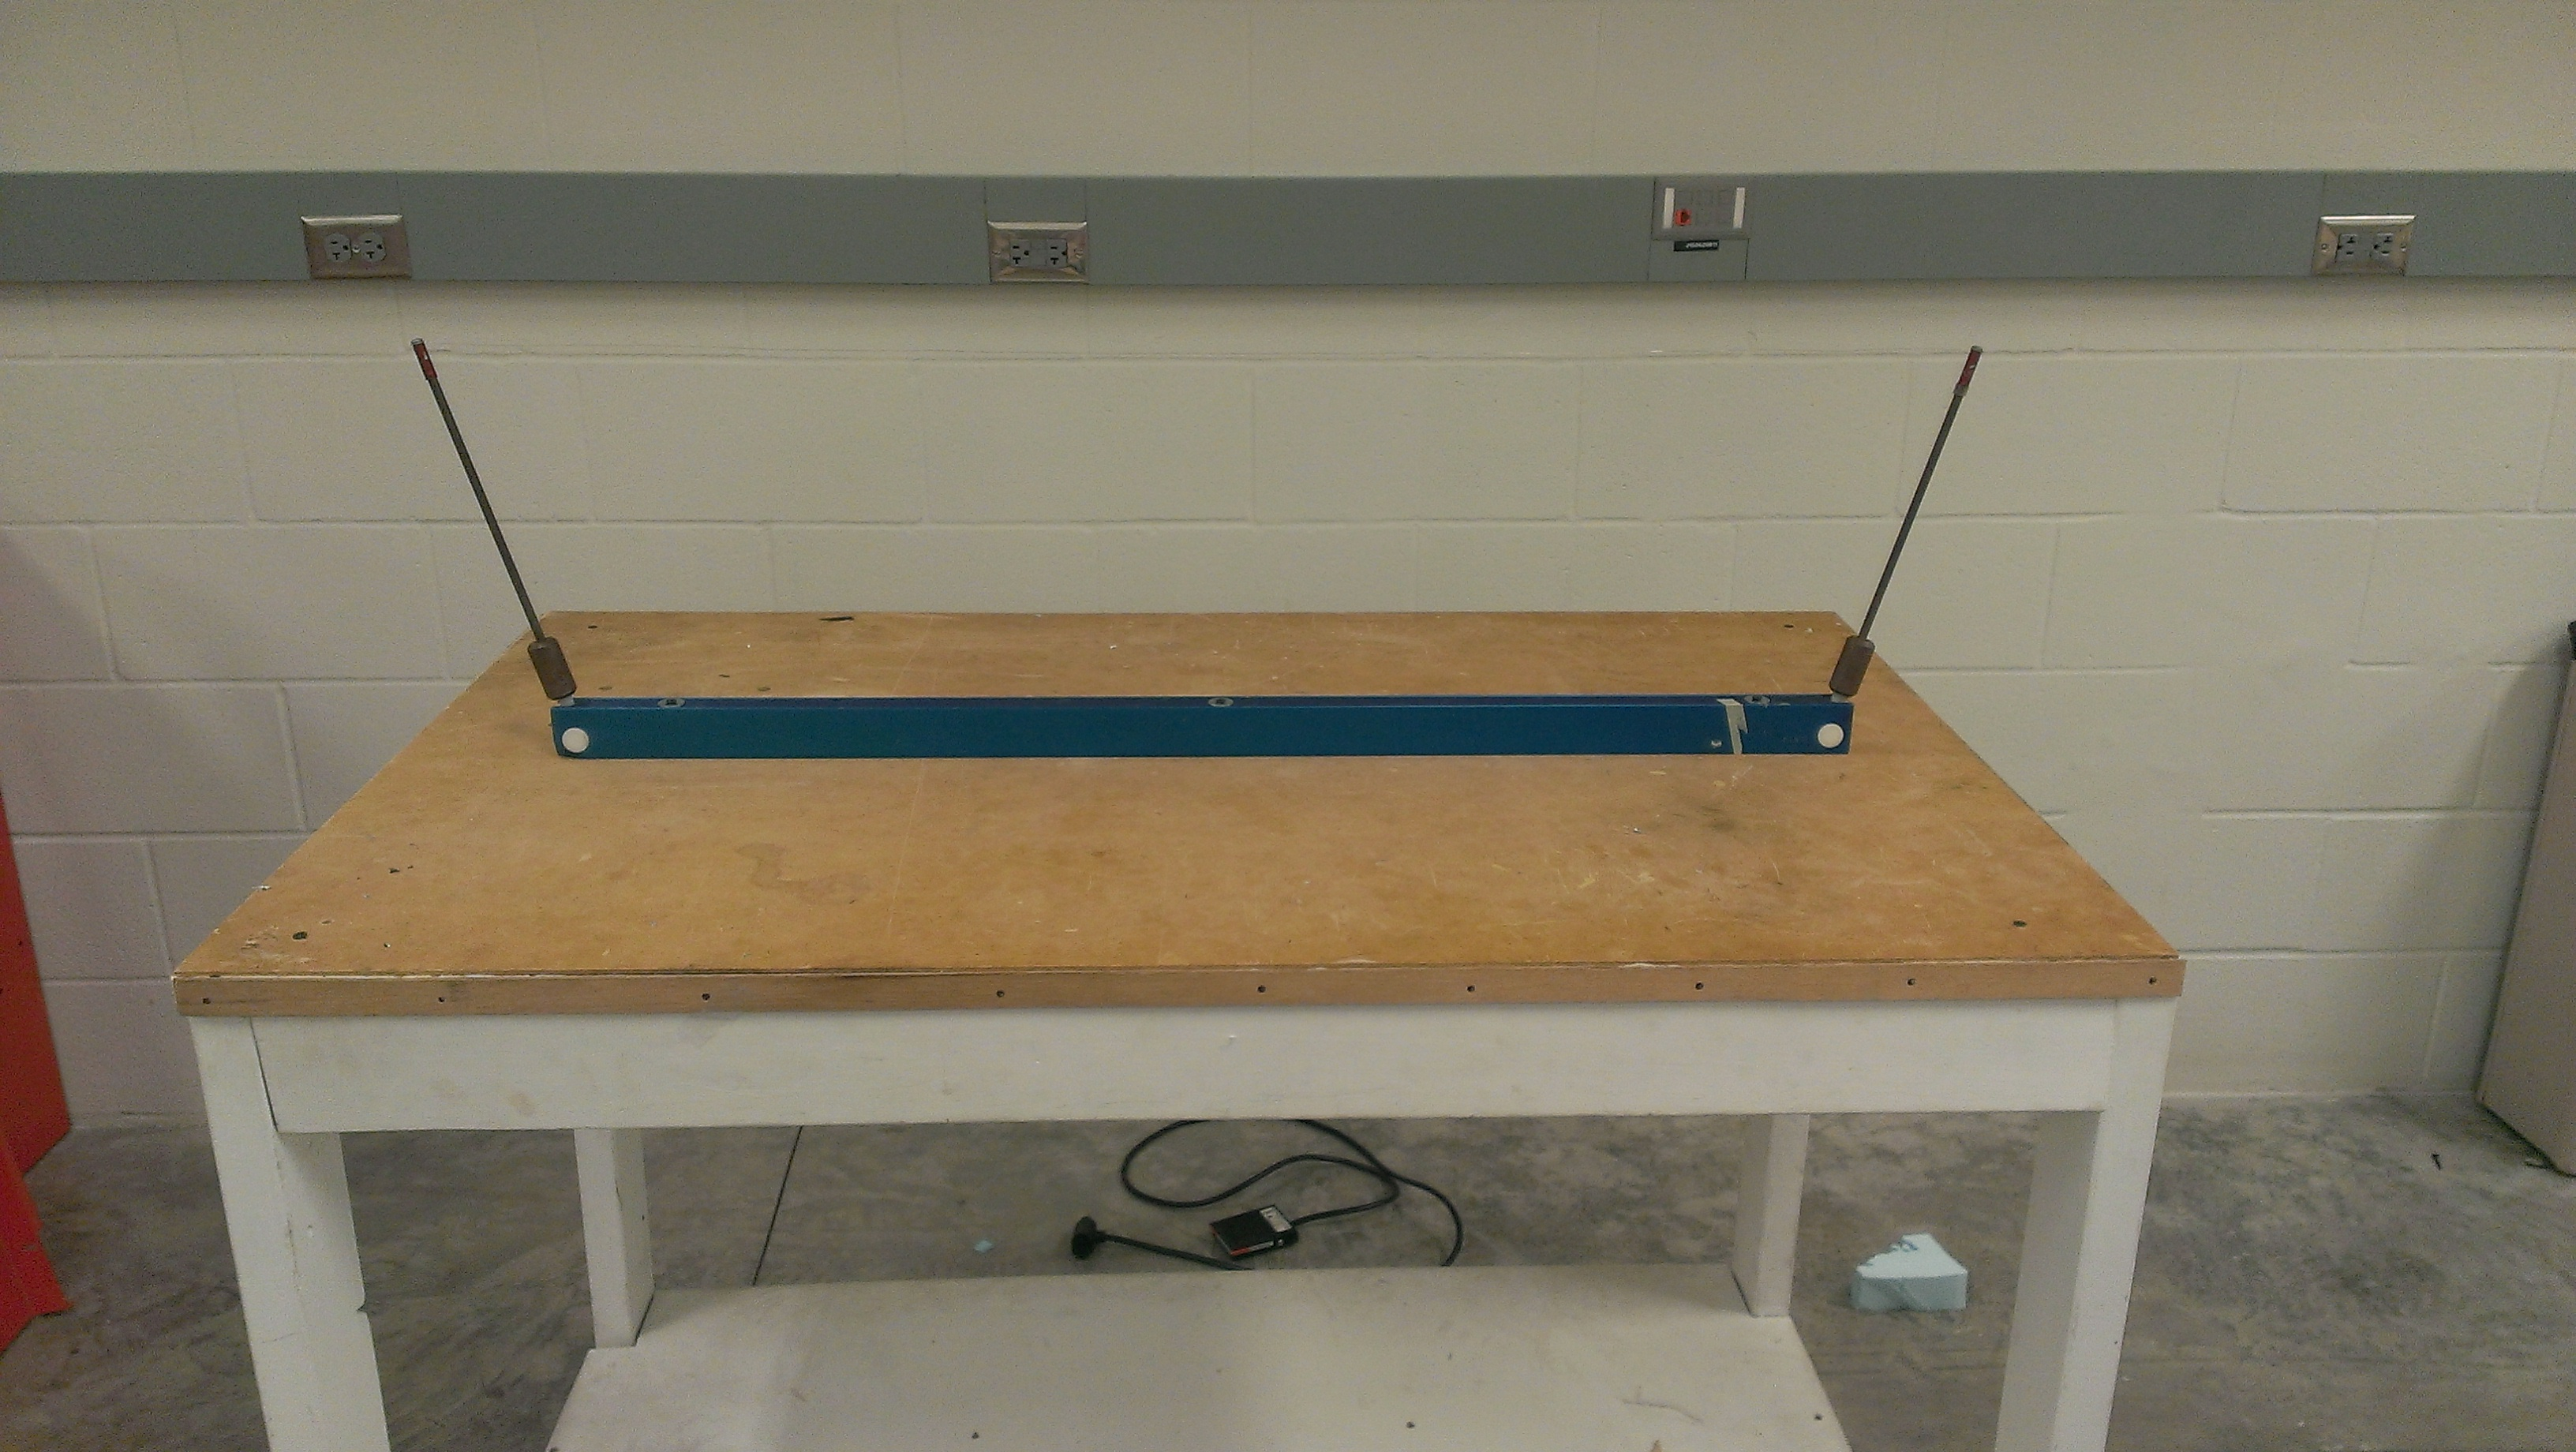
\includegraphics[width=4in]{images/IMAG0208}
\caption{Horizontal Hot Wire Cutter}
\label{fig:hortcutter}
\end{figure}

\subsection{Setup}
\begin{enumerate}
\item Ensure the hotwire is taunt, if the hotwire is not taut, loosen the top set screw and pull the wire taut and then re-tighten the set screw
\item Clip the red alligator clip to the left or right side of the wire 
\item Clip the black alligator clip to the opposite side as the red. These leads supply power to the wire
\item Plug the power unit in
\item The unit is now ready to use
\end{enumerate}
\subsection{Operation}

\begin{figure}[ht]
\centering
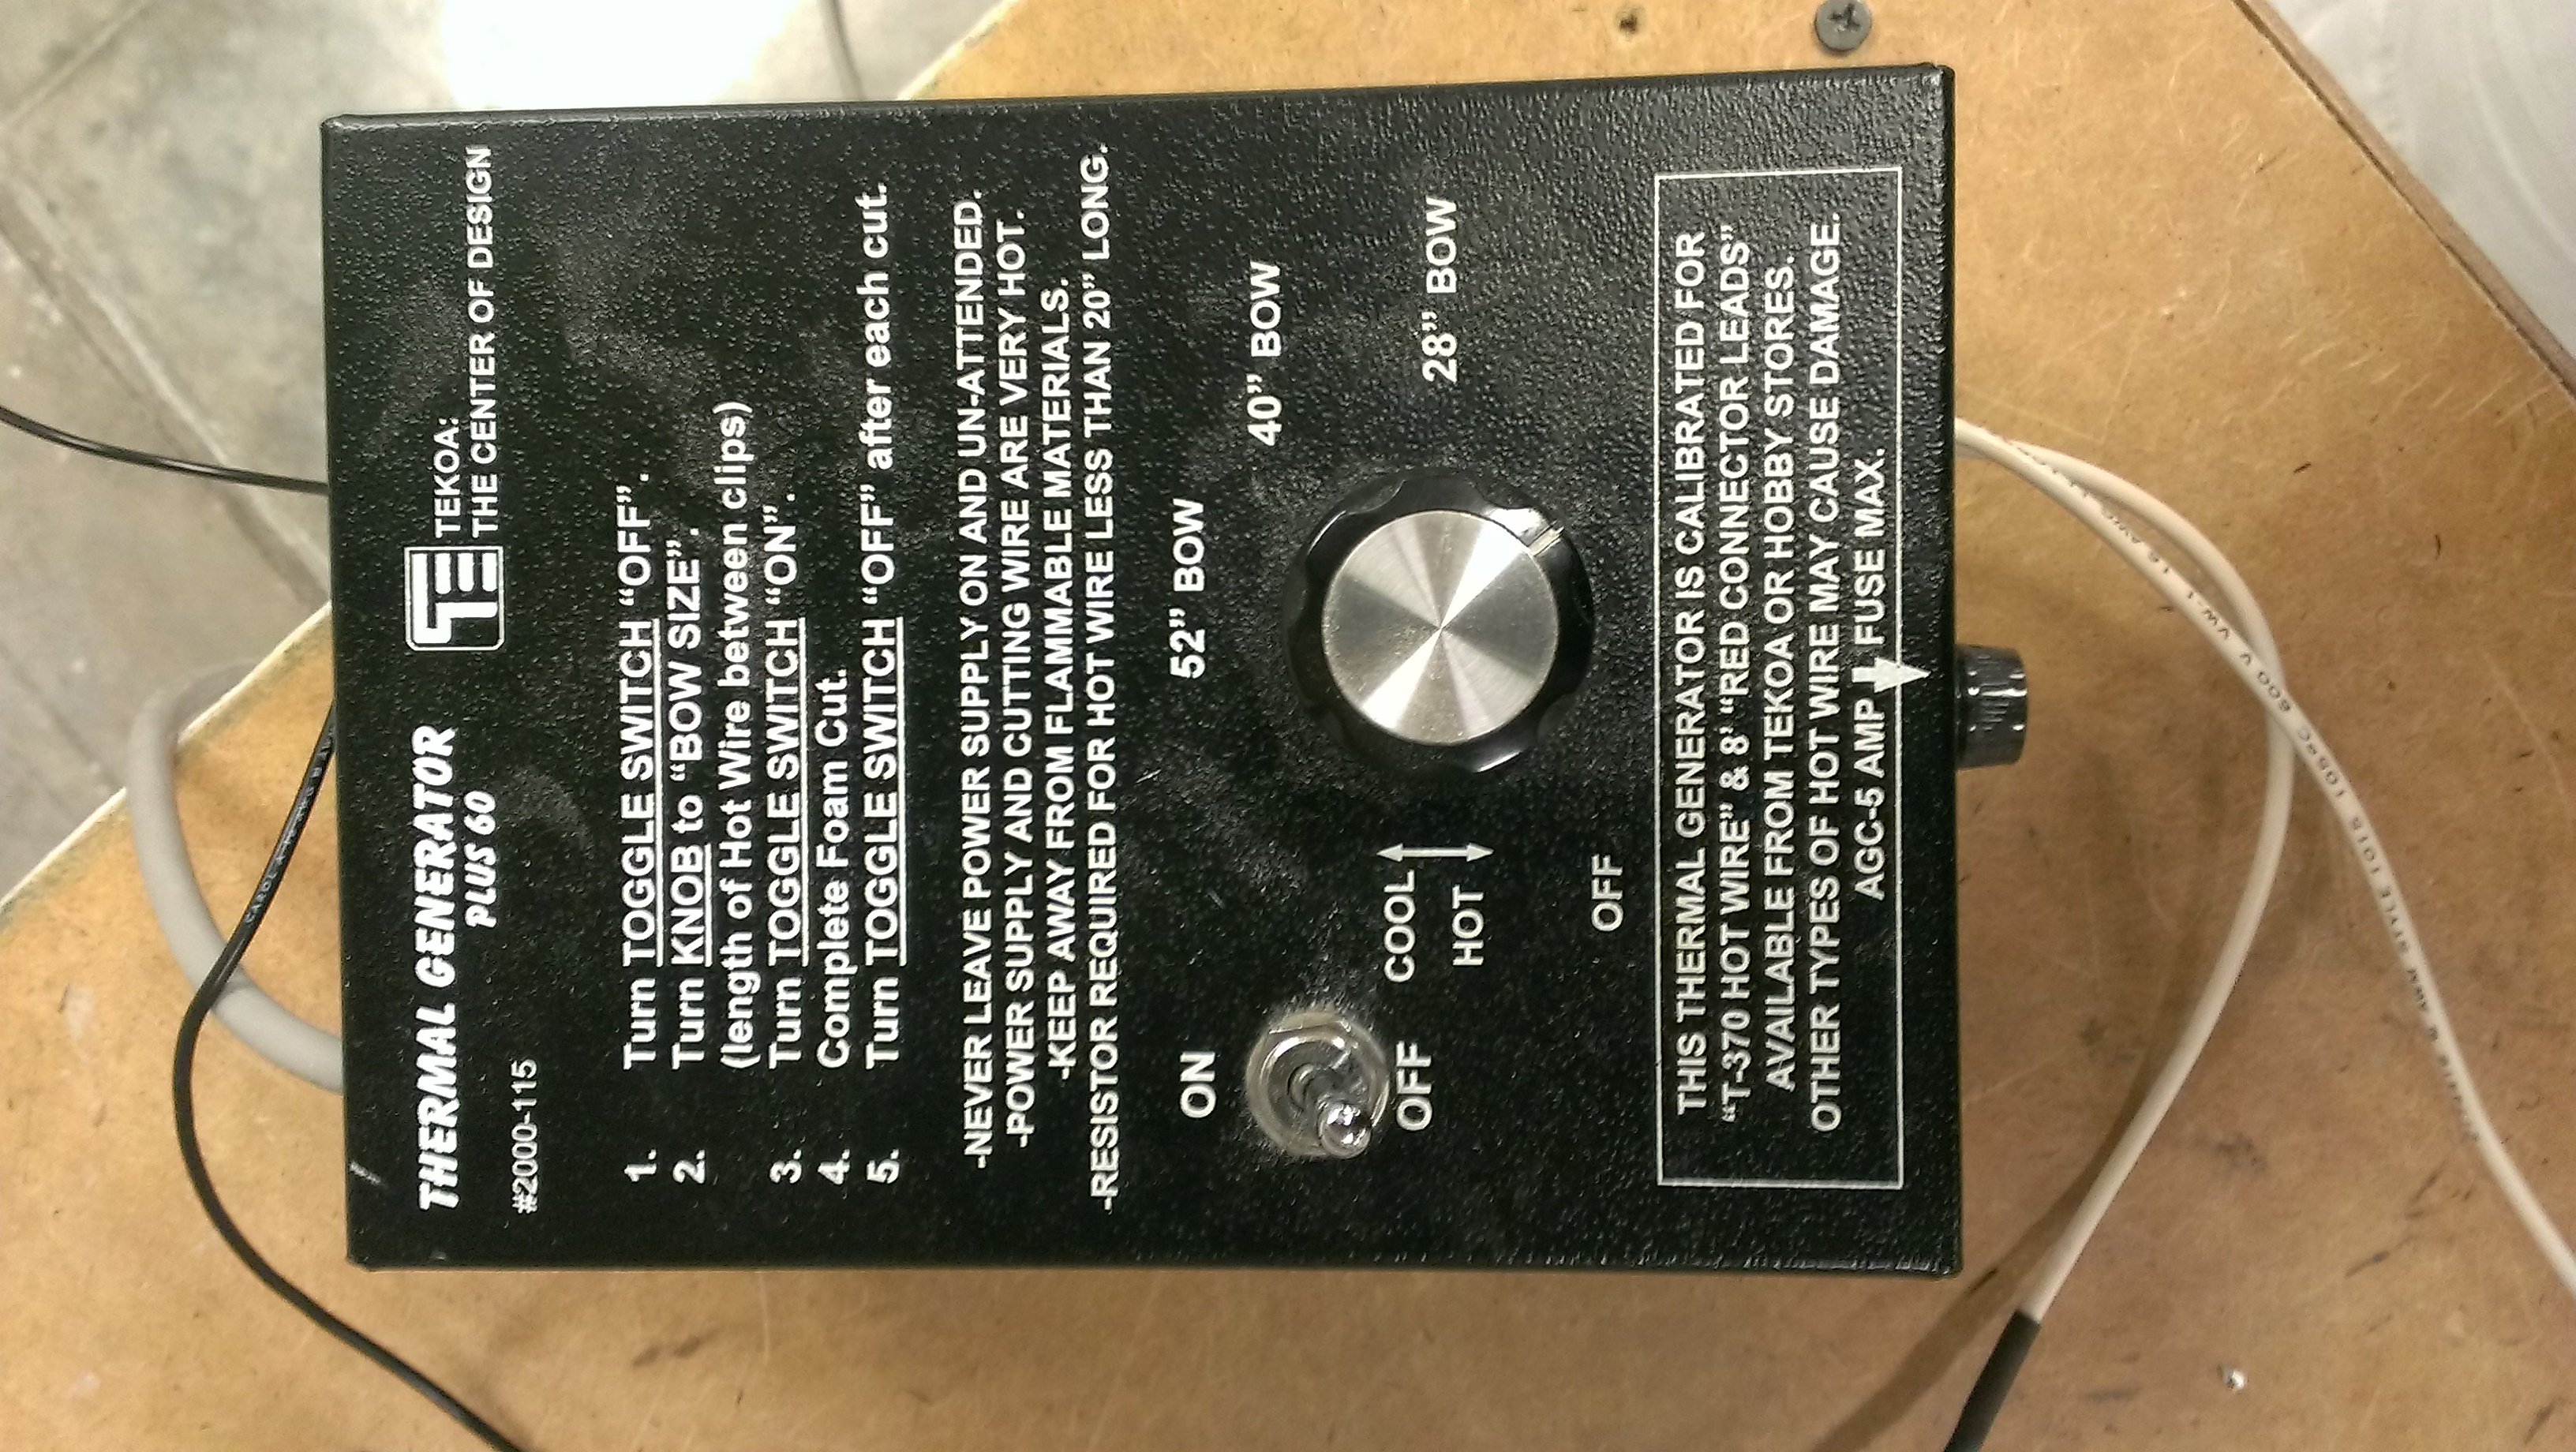
\includegraphics[angle = 270, trim = 150mm 50mm 250mm 50mm,clip,width=2in]{images/IMAG0216}
\caption{Control box for the horizontal cutter.}
\label{fig:controlbox}
\end{figure}

\begin{enumerate}
\item Set the bow size setting. This will be determined by the length of the bow itself
\item Turn the power switch into the \textbf{ON position}
\item When the wire has heated up, proceed to cut the work piece
\begin{enumerate}
\item When entering and exiting work piece, use a slow speed to prevent the wire from bowing.
\item Travel at a relatively slow pace in order to minimize wire lag
\end{enumerate}
\item When finished making cuts, turn the power off and unplug the Thermal Generator
\item Clean up immediate work area
\begin{enumerate}
\item Small, unusable foam scraps need to be thrown away
\item Excess usable foam scraps can be kept on the bottom shelf of the hot wire table
\item Sweep and vacuum after each use of the hot wire table
\end{enumerate}
\end{enumerate}

\section{Portable Hot Wire Bow}
The portable hot bow is similar in operation and purpose to the horizontal hot wire cutting station. This bow, however, it is smaller and portable.
\subsection{Setup}
\begin{enumerate}
\item Secure portable hot wire bow to an approved surface
\begin{enumerate}
\item Only the white rolling table surfaces are approved surfaces for attaching the portable hot wire
\item To secure, use two C-clamps and tighten to an exposed edge of the work surface
\end{enumerate}

\item Ensure the hotwire is taunt, if the hotwire is not taut, loosen the top set screw and pull the wire taut and then re-tighten the set screw
\item Hook up the red alligator clip of the Thermal Generator to one side of the wire and the black to the other side
\item Plug the Thermal Generator in. 
\item The portable hot wire bow is now ready to use.
\end{enumerate}
\subsection{Operation}
For operation see the Operation section of the Horizontal Hot Wire Cutting Station.
\section{Hot Knife}
Another tool for cutting foam is the hot knife which is shown in Figure \ref{fig:hotknife}. This tool operates similarly to the hot wire cutters in that it heats up a piece of metal that melts the foam. The difference is that this is a hand held tool and allows for many different complex cuts to be made.

\begin{figure}[ht]
\centering
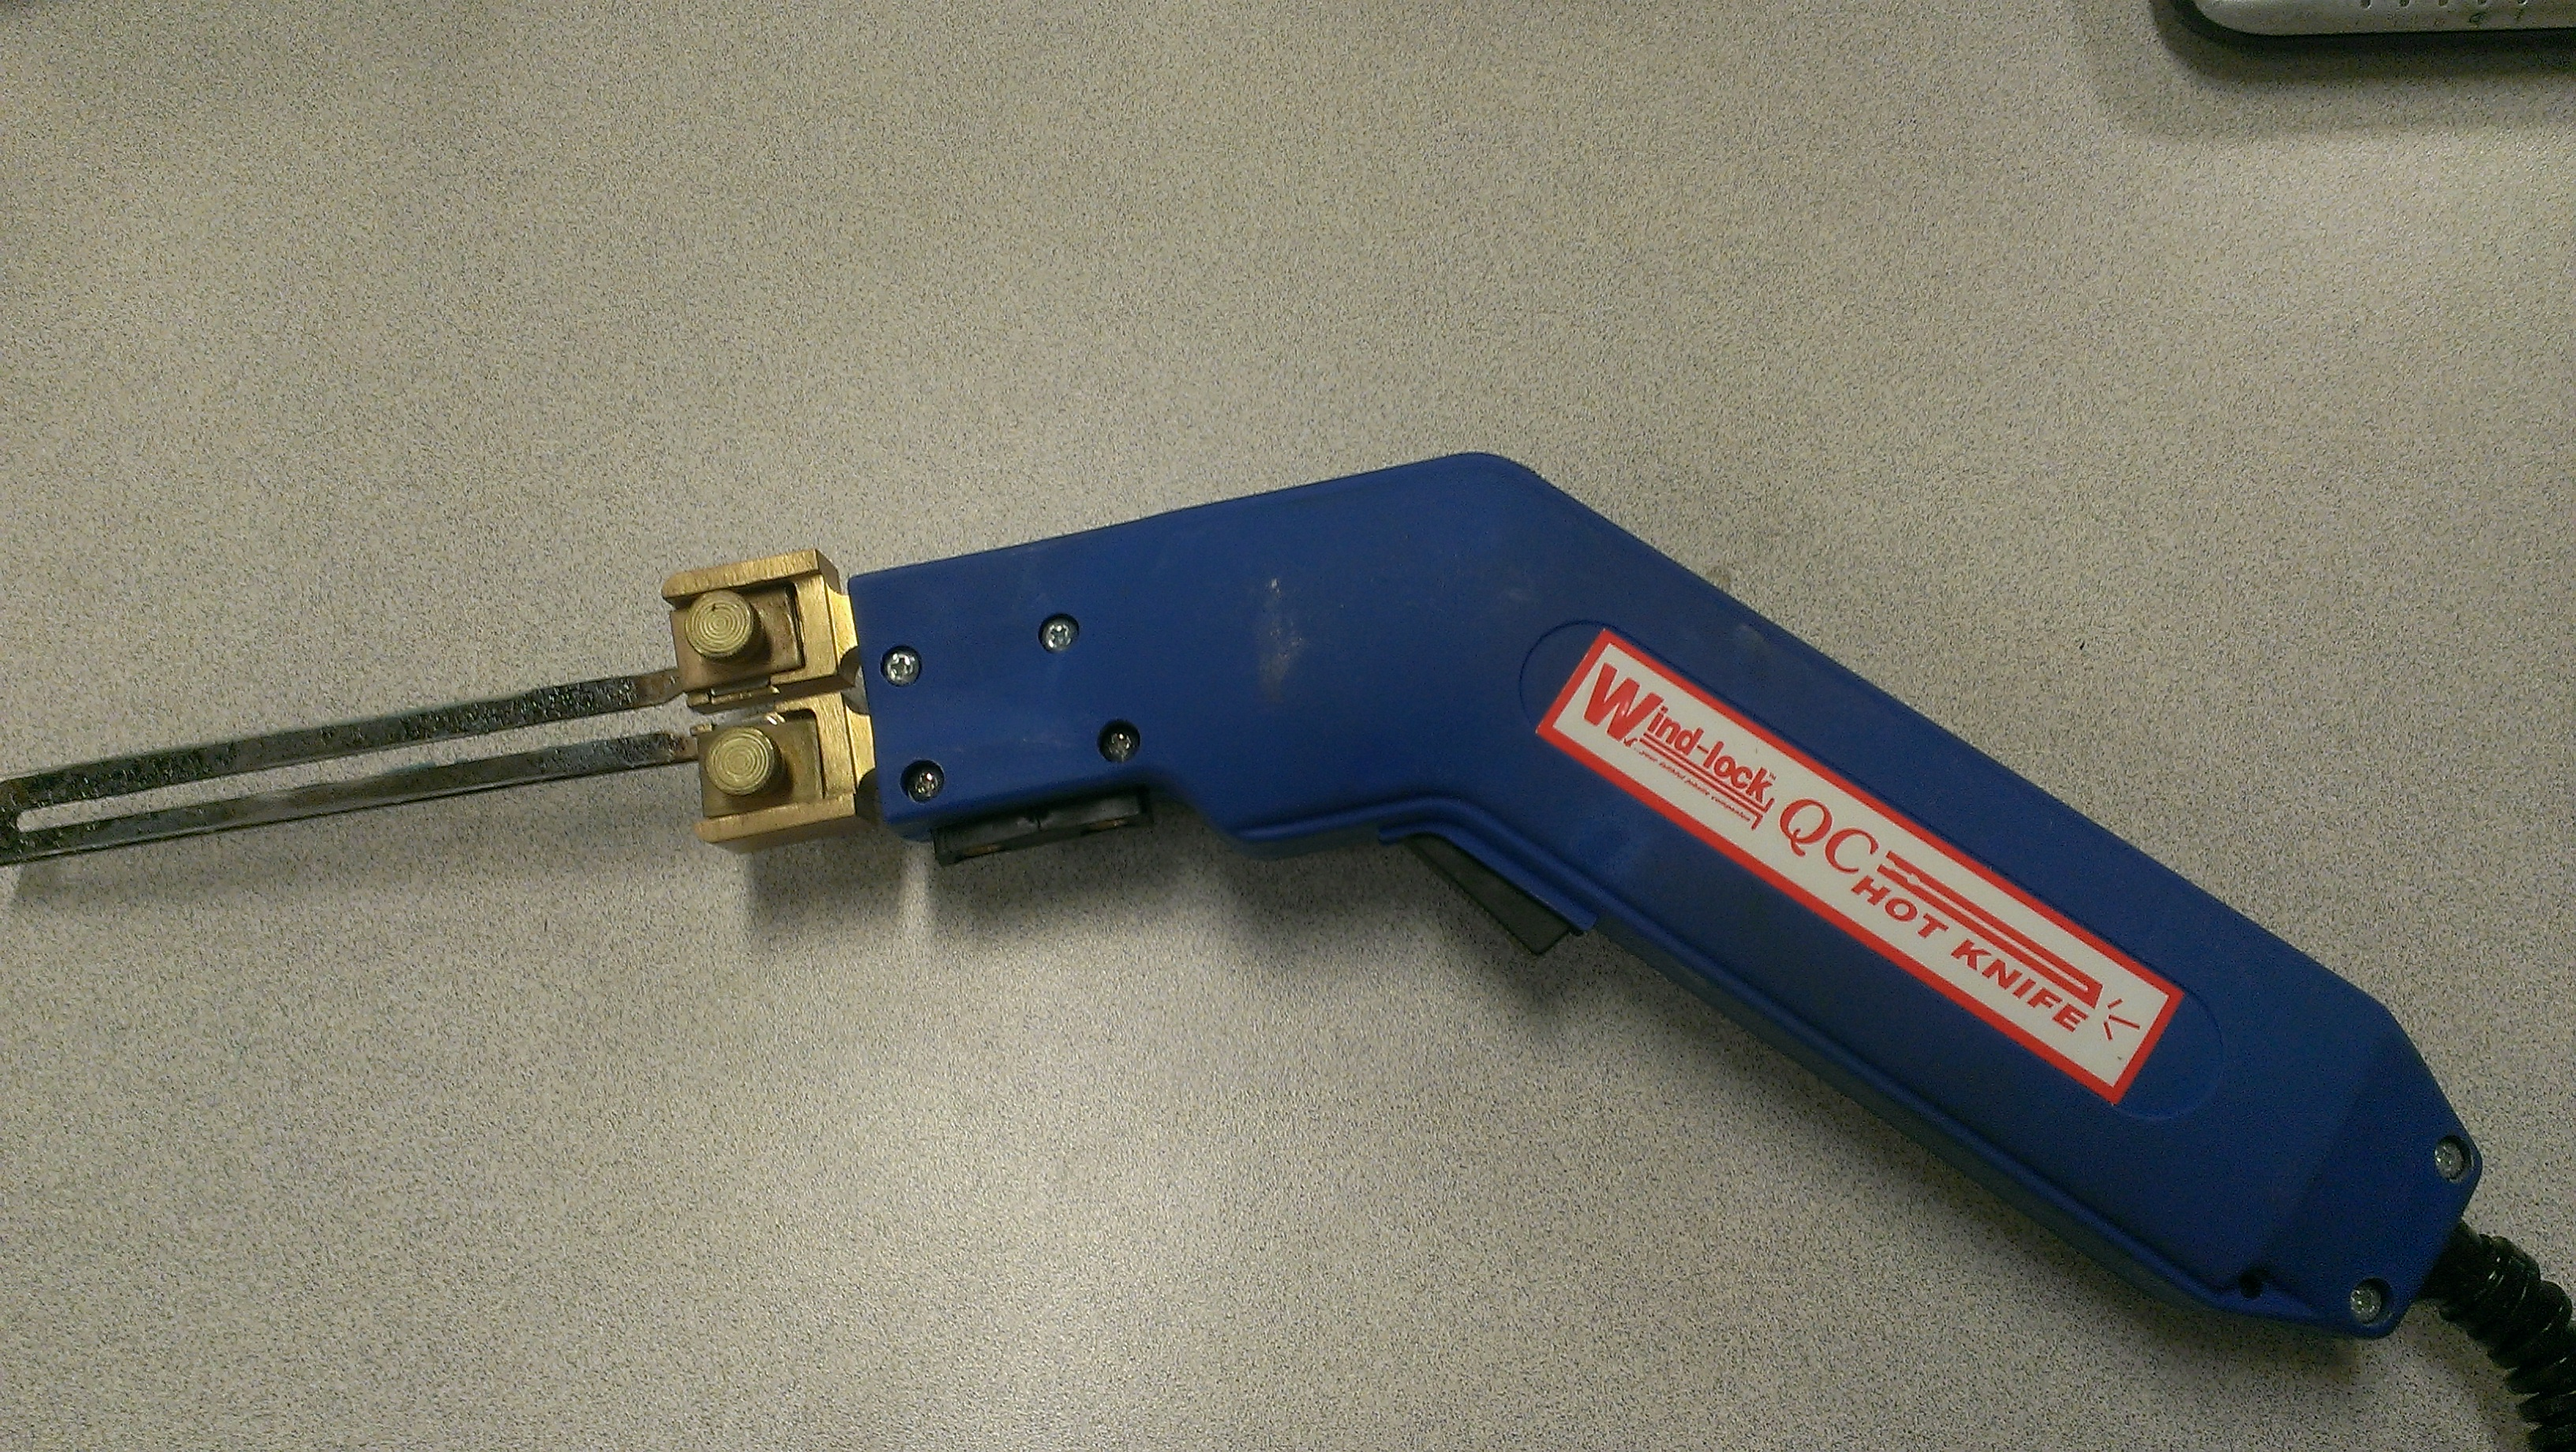
\includegraphics[width=4in]{images/IMAG0229}
\caption{Handheld hot knife}
\label{fig:hotknife}
\end{figure}

To begin using the hot knife, verify that the blade is inserted into the holder and properly secured.  In order to attach the blade, loosen the set screws, seat the blade in the grooves provided, and then tighten the set screws again.  The image below shows the blade properly seated in the hot knife.

%\begin{figure}[h]
%\centering
%\includegraphics[width=2in]{../images/IMAG0230}
%\caption{Proper seating of the blade in the hot knife.}
%\label{fig:hotwireblade}
%\end{figure}

\subsection{Basic Operation}\label{hotknife_ops}
Once the blade is secure, plug the hot knife into the outlet.  To operate the knife, press and hold the trigger.  Anytime the trigger is pulled in, the blade will quickly heat up.  Once the trigger is released, the blade will cool down.

There are two basic methods of cutting with the hot knife.  The first is to set the heat so that based off of travel rate and material, the knife cuts correctly while holding down the trigger.  The second and easier way is to turn the heat all the way up and then toggle the trigger on and off in order to achieve the desired heat in the blade.

When exiting the material, set the heat lower on the last inch or two of material so that the blade takes a bit more effort to cut with. This allows the last inch or two of material to clean off the blade of excess residue.  You should never cut with excessive heat.  Excessive heat leads to less precise cuts and also builds up melted material on the blade which ruins the blade.

When you have finished cutting your foam, ensure the blade is clean and cooled before storing.  Clean up the area immediately after done cutting and throw away any scraps.  Put away any useful pieces of foam in the proper storage area.  Vacuum and sweep up all dust and small particles that may have been generated during cutting.
\subsection{Sled Operation}

%\begin{figure}[h]
%\centering
%\includegraphics[width=2in]{../images/IMAG0233}
%\caption{The sled that may also be used with the hot knife}
%\label{fig:hotsled}
%\end{figure}
Along with the regular blade, the hot knife also comes with a sled that can make cutting straight, constant depth grooves very easy.  To use this sled, follow these steps:

\begin{enumerate}
\item Remove the blade or custom wire attachment from the hot knife.
\item Unscrew the set screws and pull the blade out.
\item Insert the sled attachment into the set screws.
\item Loosen the set screws until the attachment slides in.
\item Ensure the square metal tabs are in the correct orientation and then tighten the set screws.
\item Loosen the set screws on the front of the sled and remove the short section of custom wire.
\item Bend custom wire section to the desired profile shape and then put back into the set screw slots.
\item Tighten the set screws on the front of the sled.
\item Plug in the hot knife.
\end{enumerate}

Cutting is done in the same way as operating the hot knife with the blade attachment. See Section \ref{hotknife_ops} on cutting instructions.  Ensure the sled attachment slides evenly on the foam surface and remains in contact with the foam at all times while cutting.  When complete, ensure the blade is clean and cooled before storing.  Remove sled attachment by reversing the order used to attach it.
Make sure you clean up area immediately after done cutting and throw away scraps.  Useful pieces of foam should be properly stowed.  Vacuum and sweep the area to finish cleaning the area up.  

\subsection{Custom Wire Operation}
The hot knife cutter has another, flexible wire that allows for custom shapes to be formed.  To use the custom wire, follow the procedures below.

\begin{enumerate}
\item Bend the flexible wire into desired shape.  Avoid sharp corners and tight bends as this can ruin the wire.
\item Hook the wire into the same slots the blade attaches to.
\item Loosen set screws, attach the blade into the slots, and then tighten the set screws.
\item Plug the hot knife into an outlet.
\end{enumerate}
To operate the knife, press and hold the trigger.  There are two basic methods of cutting with the hot knife
The first is to set the heat so that based off of travel rate and material, the knife cuts correctly while holding down the trigger.

The second and easier way is to turn the heat all the way up and then toggle the trigger on and off in order to achieve the desired heat in the wire.  When exiting material, set the heat lower on the last inch or two of material so that the blade takes a bit more effort to cut with. This allows the last inch or two of material to clean off the wire of excess residue.

When using the hot knife or hot wire, never cut with excessive heat.  Excessive heat leads to less precise cuts.  Excessive heat also builds up melted material on the wire which ruins the wire.  When complete, ensure the wire is clean and cooled before storing.  When done make sure you clean up area immediately after done cutting.

\section{Sanding Foam}
\subsection{Downdraft Table}
Groups that need to sand can do so on the provided downdraft table. All sanding must be done on the downdraft table.
\begin{enumerate}
\item Turn the power switch, the left hand switch labeled power, into the ON position
\item Select the desired speed on the right hand switch labeled Speed. The up position is HIGH and the down position is LOW
\item Sand on the top surface of the machine.
\item If dust is not being pulled into the machine
\begin{enumerate}
\item Change the speed setting to HIGH if it is not already
\item If the speed is on HIGH and the dust is still not being collected, consult a lab monitor, the filter may be in need of replacement.
\end{enumerate}
\item When finished sanding, sweep any remaining dust into the collection \item system prior to turning the power off
\item Turn the power switch into the OFF position
\item Clean up the immediate area
\end{enumerate}

\subsection{Sanding Procedures}
When using procedures like CNC milling and even hot wire cutting, small defects in the material may be left over from the material removal process. In order to create a smooth, uniform finish that foam coatings can adhere to it may be necessary to sand the workpiece.  To do this, follow the steps below.

\begin{enumerate}
\item Select a sandpaper grit.  Generally 100 or 150 grit sandpaper is sufficient to sand foam.
\item Sand the foam until it reaches its desired shape.
\end{enumerate}

Since foam is much softer than wood, sanding will take much less time and require less effort to sand.  Rarely will it be necessary to sand foam with sandpaper of a higher grit than 150.  For most applications, one grit should be sufficient, however for finer finishes it may be beneficial to use a second grit.

\chapter{Foam Coatings}
Groups may want to cover their foam projects in a protective layer. There are several coatings available to students that can offer increased rigidity, strength, or flexibility.
\section{Composites}
The Make to Innovate lab has access to composite materials like fiberglass and carbon fiber. Groups are able to use these materials on their projects if needed, however, there may be a cost associated with these materials.  In addition, all composites work must take place in 0638 Howe Hall and additional training is required to work with composites.

\subsection{Carbon Fiber}
Carbon fiber is a composite material that students have access to use on their projects for an additional cost. Carbon fiber is an expensive material, but it is lighter and stiffer than other materials like fiberglass. There are certain situations in which carbon fiber is an appropriate material, despite its higher cost. Projects that require a larger strength to weight ratio and more stiffness could make use of carbon fiber. Most projects, however, do not need the benefits that carbon fiber provides. Fiberglass is a perfectly suitable material for most situations.

Groups who wish to use carbon fiber need to first seek out the approval of the use of the composites lab materials from Matthew Nelson. Upon approval, students can go to the composites lab and speak to the composites lab monitor. The lab monitor will be able to point out all necessary training that needs to be completed before using the composites lab. The monitor will also be able to educate students on how best to go about coating their project in carbon fiber.

\subsection{Fiberglass}
Fiberglass is a composite coating that is relatively cheap and relatively strong. Students have access to use this material for their projects and depending on availability it may be available at no cost to the team. For most projects, fiberglass is more than sufficient to add stiffness and strength. 

In order to use fiberglass, students must get approval from Matthew Nelson prior to being able to use lab supplies. If approved, students must then seek out the help of the composites lab monitor. The composites monitor will point out all necessary training that needs to be completed as well as the best practices on how to do their composites work.

\section{Foam Coat}
Foam coat is a new material that the lab is experimenting with. It is a gypsum coating that, depending on the additive, can add strength and flexibility. This coating is water based and can be cleaned up with water, making it easier to use and less dangerous than traditional foam coatings. There are several different additives that change the properties of the foam coat. If groups want to experiment with foam coat, they can speak with a lab monitor who will help them out.

\subsection{Base Mix}
The base mix is gypsum and water that can be mixed in various thicknesses. If thinner applications are desired, more water can be added to allow for easy spreading. Thicker applications require less water and allow for a stickier coating. For complete mixing instructions, read the label and instructions.
\subsection{Boost}
Boost, when mixed in the appropriate quantities, strengthens the base material and allows for thinner applications. This means lighter overall weight and higher strength. This coating is relatively brittle and will crack if flexed much. For mixing instructions, read the label and follow directions.
\subsection{Bounce}
When mixed in the base mix, bounce creates a flexible, rubbery coating that resists cracking. This coat does not add much rigidity, but is weather resistant. For mixing instructions, please refer to the label on the product.
\subsection{Best Coating}
The best option that has been explored so far utilizes both the boost mix and the bounce mix.  Please follow the steps below for doing a best coast method.

\begin{enumerate}
\item Prepare the surface for finishing.  All cutting, sanding, and surface prep. must be done prior to coating.
\item Mix a batch of the boost material.
\item Apply the boost material in a uniform coating.  Thickness will depend on the desired strength and weight.
\item Let coating dry completely.
\item Mix a batch of bounce.
\item Apply a coat of bounce to the piece on top of the dried coat of boost.
\end{enumerate}
Thickness will depend on the desired flexibility and weight.  Layering the two coats of material will allow for a strong, flexible part.  When bent, the boost layer may crack, but the bounce layer will stretch and contain the boost.

\section{Paint}
Painting is cheap and effective way to enhance the appearance of a project. Painting foam, however, can be difficult. Spray paints and certain other paints have solvents that will also dissolve the foam. The best way to paint foam is to use water or latex based brush-on paint. The lab has these paints readily available for student use. See a lab monitor for access to the paints.